\chapter{Methodology}
\label{cp:Methodology}

  The proposed framework uses a bottom-up pipeline to
gradually infer a high-level representation of the scratches and stains from low-level features in a back cover of mobile phone image. Firstly by mean of the wavelet transform, the surface texture properties such as scratch and stain are decomposed into so-called wavelet characteristics. Then multivariate statistical approach, i.e. Hotelling $T^{2}$ control chart is utilized to monitor the mean vector of a multivariate process, which can be used to judge the existence of scratch defects in the sample image.

\section{Maximal variance of moving windows}
For the surface of the back cover of handy, we assume that the pixels of the back cover are homogeneous. Therefore, we thought of using the variance of the pixel value to extract some features to represent the surface state. 


The control charts are used spatially by moving a mask (or window) across the image and then calculating and plotting a statistic each time the mask is moved. The size of the mask depends on the expected size of the defects to be detected, with smaller defective regions requiring smaller mask sizes.~\cite{megahed2011review}Inspired by this view, we move a 10 by 10 window across the image and calculate the variance of the pixel value each time the window is moved. Then value with the largest variance in this image is taken as the desired statistic describing this image.

\section{Discrete Wavelet transform decomposition}
  The continuous wavelet transform was computed by changing the scale of the analysis window, shifting the window in time, multiplying by the signal, and integrating over all times. In the discrete case, filters of different cutoff frequencies are used to analyze the signal at different scales. The signal is passed through a series of high pass filters to analyze the high frequencies, and it is passed through a series of low pass filters to analyze the low frequencies.


%~\cite{polikarTHE WAVELET TUTORIALusing}
  The DWT [Fig.~\ref{fig:dwt}] analyzes the signal at different frequency bands with different resolutions by decomposing the signal into a coarse approximation and detail information, which are associated with low pass and highpass filters, respectively. In our case, we use Haar discrete wavelet transform as the basic function to perform signal decomposition, so that an original image is decomposed into four coefficients: one low-pass filtering coefficients (approximation coefficients) and three high-pass filtering coefficients (detail coefficients, containing the horizontal(h), vertical(v), and diagonal(d) detail coefficients) at each level.

%Here is one example demonstrated by Fig.~\ref{fig:dwt} that adapted from~\cite{hijazi2015using}. 

\begin{figure}[h]
\centering
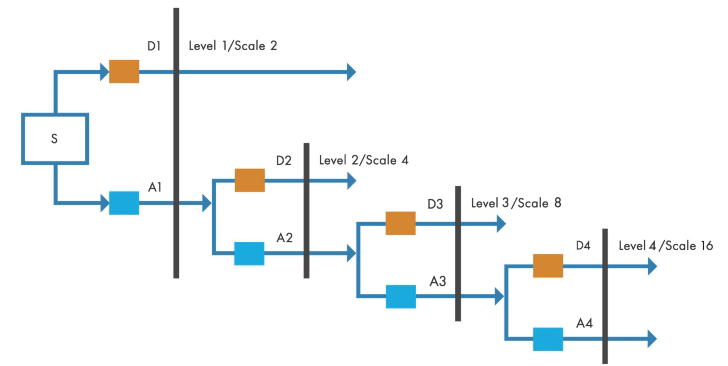
\includegraphics[width=1\textwidth]{images/dwt.png}
\caption[Structure of CNNs]{A general structure of CWT, the orange cube represent high-pass filter, the blue cube represent low-pass filter. Figure is adapted from MATLAB Tech Talks.}
\label{fig:dwt}
\end{figure}

  The number of coefficients of approximation coefficients and detail coefficients are halved when the level increase,since the images we analysized is in form of 2-D, so we need to perform the 2-D haar wavelet tranform by applying 1-D wavelet transform first on rows and then on columns.There is a built-in function in MATLAB haart2, which perform 2-D haar wavelet tranform.
the haart2 transform is obtained down to level

\begin{equation}
\log_2(min(row's dimension,column's dimension)) \label{equa:log1}
\end{equation}

 %\[\log_2(min(row's dimension,column's dimension))\] \label{equa:log1}
If the row or column dimension of data is even, but not a power of two, the haart2 transform is obtained down to level 

\begin{equation}
\lfloor \log_2(\frac{min(row's dimension,column's dimension)}{2}) \rfloor \label{equa:log2}
\end{equation}
%\[\lfloor \log_2(\frac{min(row's dimension,column's dimension)}{2}) \rfloor\] \label{equa:log2}

In our case, we have sample data of size 100 * 100, the largest level of haart2 transform is then 5 by using Equation \ref{equa:log2}.By using wavelet decomposition






\section{Wavelet decomposition based Hotteling $T^{2}$ control chart}
  In order to monitor the surface quality of the mobile phone, we need some feature quantities to characterize the quality of the image. The DWT are used to retrieved quality characteristics from image data, since It decomposes the image data into some details coefficients, which contain horizontal, vertical, and diagonal coefficients. These coefficients can be used as the input of the control chart after processing, and the control chart can then judge whether the procedure is under control by monitoring the value of the coefficient.


  A RGB image has three frame: R,G and B frame, we apply haar wavelet transform on each frame at the same time, the coefficients of final level have actually final level times filtered by high pass filter, which mean the amplitude of coefficients contain the information of high frequency signal in original image, namely The higher the coefficients, the more likely the signal will be abrupt. The Abrupt in the signal then represent the defects in the products which we are monitoring.
% maybe I should try get 9 elements to represent a image, that's more reasonable


	After we decompose an image of ($M \times N$) pixels, we get horizontal(h), vertical(v), and diagonal(d) coefficient matrix($S \times S$) for each frame at final level($L$),each coefficient matrix have $S^2$ coefficients,an image sample can have $3 \times S^2$ coefficients.~\ref{montgomery2020introduction} present tables indicating the recommended number of quality characteristics p = 2, 3, 4, 5, 10, and 20. It turns out that the cooeficients of dianonal coefficient matrix can best reflects the surface defects of various shapes(see experiment ~\ref{cp:experiment}),thus we first absolute all coefficients, which turn negative coefficients into positive coefficients withoud changing the value of itself. After that we take the maximal coefficient among the diagonal matrix and consider it as the disired statistical charateristic of coresponding frame. Finally 3 coefficients retrieved from an image is composing the mean characteristic vector in Multivariate Control Chart. 


There are two distinct phases of the control chart~\cite{bersimis2007multivariate}.

\begin{itemize}
\item Phase I: charts are used for retrospectively testing whether the process was in control when the first
subgroups were being drawn. In this phase, the charts are used as aids to the practitioner, in bringing a
process into a state where it is statistically in control.
\item Phase II: control charts are used for testing whether the process remains in control when future subgroups
are drawn. In this phase, the charts are used as aids to the practitioner in monitoring the process for any
change from an in-control state.
\end{itemize}

Multivariate Control Chart can be utilized to simultaneous monitor more than one quality characteristic. 




